\documentclass[conference]{IEEEtran}
\IEEEoverridecommandlockouts
% The preceding line is only needed to identify funding in the first footnote. If that is unneeded, please comment it out.
%Template version as of 6/27/2024

\usepackage{float}
\usepackage{cite}
\usepackage{amsmath,amssymb,amsfonts}
\usepackage{algorithmic}
\usepackage{graphicx}
\usepackage{textcomp}
\usepackage{xcolor}
\usepackage[dvipsnames]{xcolor}
\usepackage{hyperref}
\usepackage[utf8]{inputenc}
\usepackage[greek,english]{babel}
\usepackage{alphabeta}
\hypersetup{colorlinks=true, linkcolor=black, urlcolor=black, citecolor=black}

\def\BibTeX{{\rm B\kern-.05em{\sc i\kern-.025em b}\kern-.08em
    T\kern-.1667em\lower.7ex\hbox{E}\kern-.125emX}}
\begin{document}

\title{HomeSense: Συλλογή και Οπτικοποίηση Περιβαλλοντικών Δεδομένων}

\author{
	\IEEEauthorblockN{Ιορδάνης Κωστελίδης}
	\IEEEauthorblockA{
		\textit{Πρόγραμμα Μεταπτυχιακών Σπουδών στη Ρομποτική}\\
		\textit{Τμήμα Μηχανικών Πληροφορικής, Υπολογιστών και Τηλεπικοινωνιών}\\
		\textit{Σχολή Μηχανικών}\\
		\textit{Διεθνές Πανεπιστήμιο της Ελλάδος}\\
		Σέρρες, Ελλάδα \\
		iordkost@ihu.gr
	}
}

\maketitle

\begin{abstract}
	Το HomeSense αποτελεί ένα ολοκληρωμένο σύστημα συλλογής και οπτικοποίησης περιβαλλοντικών δεδομένων. Το σύστημα ενσωματώνει στην τρέχουσα έκδοσή του, τρεις ειδικά σχεδιασμένες συσκευές (GasSense, LightSense, TempSense) βασισμένες στο λογισμικό NodeSense το οποίο είναι συμβατό με το NodeMCU ESP8266, οι οποίες μέσω WiFi, προσφέρουν τα δεδομένα του αισθητήρα τους μέσω HTTP API. Ο κεντρικός κόμβος, αποτελείται από 2 εφαρμογές (συλλογής και οπτικοποίησης δεδομένων) οι οποίες εκτελούνται πάνω σε Raspberry Pi 3B+ μέσω της πλατφόρμας Docker Compose.\\
\end{abstract}

\begin{IEEEkeywords}
	HomeSense, GasSense, LightSense, TempSense, NodeSense, NodeMCU ESP8266, WiFi, HTTP API, Raspberry Pi 3B+, Docker, Docker Compose
\end{IEEEkeywords}

\section{Εισαγωγή}
Το HomeSense βασίζεται σε μια αρθρωτή αρχιτεκτονική που περιλαμβάνει, τρεις ειδικά σχεδιασμένες συσκευές όπου η κάθε μια έχει από έναν αισθητήρα, και έναν κεντρικό κόμβο συλλογής και οπτικοποίησης δεδομένων. Αναλυτικά, για τις συσκευές, έχουμε μετρητή συγκέντρωσης αερίων, έντασης φωτός αλλά και θερμοκρασίας. Οι συσκευές αυτές βασίζονται στο NodeMCU ESP8266, καθώς αυτός υποστηρίζει επικοινωνία μέσω WiFi και μπορεί να διαθέσει δεδομένα μέσω HTTP APIs. Καθώς οι 3 αυτές συσκευές έχουν κοινά χαρακτηριστικά (σύνδεση σε WiFi, ίδια HTTP API End-Points), έγινε η ανάπτυξη ενός πρότυπου (template) λογισμικού, με την ονομασία NodeSense.

\begin{figure}[H]
	\centerline{\includegraphics[width=0.5\textwidth]{assets/index-html}}
	\caption{Εικόνα του HomeSenseUI.}
	\label{Εικόνα του HomeSenseUI.}
\end{figure}

Ο κεντρικός κόμβος, υλοποιείται σε Raspberry Pi 3B+, ο οποίος συλλέγει τα δεδομένα από τις συσκευές, τα αποθηκεύει σε μια βάση δεδομένων και τα καθιστά διαθέσιμα για οπτικοποίηση από τον χρήστη.

\section{Σκοπιμότητα}
Συνδυάζοντας την ευελιξία του Raspberry Pi 3B+ με τρεις ειδικά διαμορφωμένες συσκευές οι οποίες αξιοποιούν αισθητήρες μέτρησης συγκέντρωσης αερίων στην ατμόσφαιρα, έντασης φωτός αλλά και θερμοκρασίας, προσφέρουν τις μετρήσεις τους μέσω WiFi μέσω μιας διεπαφής HTTP API. Έτσι επιτρέπει τη συνεχή και αυτοματοποιημένη συλλογή δεδομένων, την αποθήκευσή τους σε μια βάση δεδομένων αλλά και την γραφιστική απεικόνισή τους μέσω μιας διαδικτυακής εφαρμογής.

\subsection{Εφαρμογές του Συστήματος}
\begin{enumerate}
	\item Οικιακή χρήση: Μπορεί να χρησιμοποιηθεί για την παρακολούθηση περιβαλλοντικών συνθηκών στο σπίτι. Για παράδειγμα, ο αισθητήρας αερίων (MQ-6) μπορεί να εντοπίσει διαρροές υγραερίου, ο αισθητήρας φωτός (LDR) να αξιολογήσει το φωτισμό σε χώρους, και ο αισθητήρας θερμοκρασίας (DS18B20) να καταγράψει τις θερμοκρασίες για να διασφαλιστεί μια άνετη διαβίωση.
	\item Βιομηχανική χρήση: Σε βιομηχανικούς χώρους, το σύστημα μπορεί να συμβάλει στην ανίχνευση επικίνδυνων συνθηκών, όπως αυξημένα επίπεδα επικίνδυνων αερίων ή ανεπαρκή φωτισμό.
	\item Έξυπνες Πόλεις: Μπορεί να αποτελέσει μέρος μιας ευρύτερης πλατφόρμας για την παρακολούθηση περιβαλλοντικών συνθηκών, ενισχύοντας τις λύσεις για την ποιότητα ζωής σε αστικά περιβάλλοντα.
	\item Ιατρικές Εφαρμογές: Στον τομέα της υγείας, μπορεί να προσφέρει σημαντική αξία καθώς:
	      \begin{enumerate}
	      	\item Οι γιατροί μπορούν να δουν αν ο ασθενής εκτέθηκε σε επικίνδυνες συγκεντρώσεις αερίου, όπως υγραέριο, και να εκτιμήσουν το βαθμό της έκθεσης.
	      	\item Το σύστημα μπορεί να καταγράψει μετρήσεις θερμοκρασίας του χώρου, παρέχοντας στους γιατρούς στοιχεία για πιθανές επιπτώσεις στην υγεία του ασθενούς λόγω παρατεταμένης έκθεσης σε χαμηλές ή υψηλές θερμοκρασίες.
	      \end{enumerate}	
\end{enumerate}

\subsection{Σημαντικότητα της Εφαρμογής}
Η ανάπτυξη ενός τέτοιου συστήματος είναι σημαντική για πολλούς λόγους:
\begin{enumerate}
	\item Ασφάλεια: Μπορεί σε μελλοντική έκδοση να ειδοποιεί έγκαιρα, τον χρήστη αλλά και αρμόδιους φορείς (π.χ. ΕΚΑΒ), για επικίνδυνες καταστάσεις, όπως διαρροές υγραερίου, προστατεύοντας ανθρώπινες ζωές.
	\item Εξοικονόμηση Ενέργειας: Η καταγραφή δεδομένων φωτός και θερμοκρασίας μπορεί σε μελλοντική έκδοση να βοηθήσει στην εξοικονόμηση ενέργειας μέσω βελτιστοποιημένης χρήσης φωτισμού και συστημάτων κλιματισμού.
\end{enumerate}

\subsection{Επεκτασιμότητα}

Μπορεί να χρησιμοποιηθεί σε πολλές άλλες περιπτώσεις, όπως:
\begin{enumerate}
	\item Γεωργία: Με προσθήκη αισθητήρων εδάφους και υγρασίας, το σύστημα μπορεί να παρακολουθεί τις συνθήκες καλλιέργειας.
	\item Ιατρική:  Καταγραφή περιβαλλοντικών παραγόντων για ασθενείς με χρόνια προβλήματα υγείας.
	\item Εκπαίδευση: Μπορεί να λειτουργήσει ως βάση για μελλοντικά projects φοιτητών σε θέματα IoT, λογισμικού, και αυτοματισμού.
\end{enumerate}

Με αυτόν τον τρόπο, αναδεικνύεται ως μια πολυχρηστική πλατφόρμα, με δυνατότητες προσαρμογής σε πολλούς τομείς της καθημερινότητας και της βιομηχανίας.

\section{Προδιαγραφές του Συστήματος}

Το σύστημα που υλοποιείται έχει ως στόχο την ασύρματη διασύνδεση μικροελεγκτών με ένα Raspberry Pi 3B+ για την καταγραφή και παρουσίαση δεδομένων από τρεις αισθητήρες. Οι δύο αισθητήρες είναι αναλογικοί, ενώ ο τρίτος είναι ψηφιακός. Η διασύνδεση πραγματοποιείται μέσω WiFi, εξασφαλίζοντας την ευελιξία και την αξιοπιστία στη μετάδοση δεδομένων. Παρακάτω περιγράφονται οι προδιαγραφές του συστήματος, όπως καθορίστηκαν από το προτεινόμενο θέμα και τις αποφάσεις που πάρθηκαν κατά τη σχεδίαση.

\subsection{Αρχιτεκτονική του Συστήματος}

\begin{itemize}
	\item \textbf{Ασύρματη Διασύνδεση}:  
	      Η επικοινωνία μεταξύ των ειδικά διαμορφωμένων συσκευών και του Raspberry Pi γίνεται μέσω WiFi χρησιμοποιώντας το πρωτόκολλο HTTP. Κάθε μικροελεγκτής διαθέτει την δική του διεύθυνση IP και παρέχει HTTP API για την διάθεση των δεδομένων του αισθητήρα του.
	      	      
	\item \textbf{Ειδικά σχεδιασμένες συσκευές με ESP8266}:  
	      Οι ειδικά σχεδιασμένες συσκευές υλοποιούν το λογισμικό NodeSense, το οποίο έχει σχεδιαστεί για τον μικροελεγκτή NodeMCU (ESP8266) και είναι οι εξής:
	      \begin{itemize}
	      	\item \textbf{GasSense}: Χρησιμοποιεί τον αισθητήρα MQ-6 (αναλογικός) για την μέτρηση αερίων.
	      	\item \textbf{LightSense}: Χρησιμοποιεί τον αισθητήρα LDR (αναλογικός) για τη μέτρηση φωτεινότητας.
	      	\item \textbf{TempSense}: Χρησιμοποιεί τον αισθητήρα DS18B20 (ψηφιακός) για την μέτρηση θερμοκρασίας.
	      \end{itemize}
	      	      
	\item \textbf{Raspberry Pi 3B+}:  
	      Το Raspberry Pi λειτουργεί ως κεντρικός κόμβος, όπου εκτελώντας 2 εφαρμογές, μπορεί:
	      \begin{itemize}
	      	\item Να λάβει δεδομένα από τις συσκευές κάθε 5 δευτερόλεπτα.
	      	\item Να αποθηκεύσει τα δεδομένα σε βάση δεδομένων.
	      	\item Να παρουσιάσει τα δεδομένα στον χρήστη.
	      \end{itemize}
\end{itemize}

\subsection{Δυνατότητες του Τελικού Συστήματος}

\begin{enumerate}
	\item \textbf{Καταγραφή Δεδομένων Αισθητήρων}:  
	      \begin{itemize}
	      	\item Συλλογή δεδομένων αερίου, φωτεινότητας και θερμοκρασίας.
	      	\item Διάθεση των δεδομένων μέσω του πρωτοκόλλου HTTP.
	      \end{itemize}
	      	      
	\item \textbf{Διαχείριση και Αποθήκευση Δεδομένων}:  
	      \begin{itemize}
	      	\item Μια Java/Spring Boot εφαρμογή που τρέχει στο Raspberry Pi 3B+, όπου μπορεί:
	      	      \begin{itemize}
	      	      	\item Να αποθηκεύει τις μετρήσεις των αισθητήρων σε βάση δεδομένων Postgres. 
	      	      	\item Να αποθηκεύει τις μετρήσεις των αισθητήρων μέσω χρονοπρογραμματισμένης λήψης δεδομένων (κάθε 5 δευτερόλεπτα).
	      	      \end{itemize}
	      \end{itemize}
	      	      
	\item \textbf{Παρουσίαση Δεδομένων}:  
	      \begin{itemize}
	      	\item Μια JavaScript εφαρμογή, όπου ο χρήστης μπορεί:
	      	      \begin{itemize}
	      	      	\item Να εντοπίζει συμβατές συσκευές στο δίκτυό του
	      	      	\item Να προσθέτει συμβατές συσκευές από το δίκτυό του
	      	      	\item Να βλέπει σε πραγματικό χρόνο τις μετρήσεις των αισθητήρων των συσκευών του
	      	      \end{itemize}
	      \end{itemize}
	      	      
	\item \textbf{Επεκτασιμότητα}:  
	      Το σύστημα είναι σχεδιασμένο ώστε να μπορεί να επεκταθεί με προσθήκη νέων συσκευών/αισθητήρων, καθώς λειτουργεί με βάση το HTTP API που έχει καθοριστεί από το NodeSense template.
\end{enumerate}

\subsection{Συνοπτική Περιγραφή Λειτουργικότητας}

\begin{enumerate}
	\item Ο χρήστης εγκαθιστά το HomeSense στο Raspberry Pi του.
	\item Ο χρήστης συνδέει στο ρεύμα τις συσκευές του.
	\item Ο χρήστης εντοπίζει μέσω του HomeSenseUI τις IP διευθύνσεις των συσκευών του.
	\item Ο χρήστης προσθέτει μέσω του HomeSenseUI τις συσκευές του.
	\item Το Raspberry Pi 3B+ πραγματοποιεί περιοδικά αιτήματα στα HTTP API των συνδεδεμένων συσκευών για τη λήψη δεδομένων.
	\item Ο χρήστης βλέπει μέσω του HomeSenseUI, τα δεδομένα σε μορφή γραφημάτων.
\end{enumerate}

\section{Λίστα υλικών}

Η σχεδίαση του συστήματος βασίστηκε σε συγκεκριμένα υλικά που επιλέχθηκαν με κριτήριο την απόδοση, το κόστος και την ευκολία υλοποίησης. Παρακάτω παρουσιάζονται αναλυτικά τα υλικά.

\subsection{Carbon Film Resistor Kit}

\begin{figure}[H]
	\centerline{\includegraphics[width=0.2\textwidth]{assets/resistorkit}}
	\caption{Εικόνα του Carbon Film Resistor Kit .}
	\label{Εικόνα του Carbon Film Resistor Kit .}
\end{figure}

Το Carbon Film Resistor Kit, είναι ένα πακέτο με αντιστάσεις διαφόρων τιμών. Κάθε Kit έχει 250 αντιστάσεις. Το κόστος του είναι περίπου €3 ανά kit. \cite{resistorkit}

\subsection{ESP8266 (NodeMCU)}

\begin{figure}[H]
	\centerline{\includegraphics[width=0.2\textwidth]{assets/nodemcu.jpg}}
	\caption{Εικόνα του NodeMCU ESP8266.}
	\label{Εικόνα του NodeMCU ESP8266.}
\end{figure}

Το NodeMCU (ESP8266) χρησιμοποιήθηκε για κάθε μια από τις τρεις συσκευές. Είναι εξοπλισμένο με ενσωματωμένο WiFi για την ασύρματη διασύνδεση με το Raspberry Pi. Το κόστος του είναι περίπου €7 ανά μονάδα, καθιστώντας το ιδανική επιλογή για οικονομική υλοποίηση. \cite{esp8266}  Οι αναλογικές τιμές από τους αισθητήρες GasSense και LightSense μετατρέπονται από το ADC \cite{adc} του ESP8266, ενώ οι ψηφιακές τιμές από το TempSense συλλέγονται μέσω του πρωτοκόλλου 1-Wire \cite{ds18b20-1wire}.

\subsection{MQ-6 (Gas Sensor)}

\begin{figure}[H]
	\centerline{\includegraphics[width=0.2\textwidth]{assets/gas}}
	\caption{Εικόνα του MQ-6.}
	\label{Εικόνα του MQ-6.}
\end{figure}

Ο αισθητήρας MQ-6 είναι αναλογικός και ανιχνεύει εύφλεκτα αέρια, όπως το LPG και το προπάνιο. Η αντίστασή του μεταβάλλεται ανάλογα με τη συγκέντρωση του αερίου στον αέρα. Το κόστος του είναι περίπου €3 ανά μονάδα. \cite{mq6}

\subsection{LDR (Photo Resistor)}

\begin{figure}[H]
	\centerline{\includegraphics[width=0.2\textwidth]{assets/light}}
	\caption{Εικόνα του LDR.}
	\label{Εικόνα του LDR.}
\end{figure}

Ο αισθητήρας LDR βασίζεται στη μεταβολή της αντίστασής του ανάλογα με την ένταση του φωτός. Το κόστος του είναι περίπου €0.20 ανά μονάδα και επιλέχθηκε λόγω της απλότητας και του χαμηλού κόστους . \cite{ldr}

\subsection{DS18B20 (Temperature Sensor)}

\begin{figure}[H]
	\centerline{\includegraphics[width=0.2\textwidth]{assets/temp}}
	\caption{Εικόνα του DS18B20.}
	\label{Εικόνα του DS18B20.}
\end{figure}

Ο αισθητήρας DS18B20 είναι ψηφιακός και χρησιμοποιεί το πρωτόκολλο 1-Wire για την επικοινωνία. Παρέχει άμεση μέτρηση θερμοκρασίας σε ψηφιακή μορφή, με εύρος μέτρησης -55°C έως +125°C και ακρίβεια ±0.5°C από -10°C έως +85°C. Η τάση λειτουργίας του κυμαίνεται από 3.0V έως 5.5V. Το κόστος του είναι περίπου €3.60 ανά μονάδα. Επιλέχθηκε λόγω της υψηλής ακρίβειας και της ευκολίας επικοινωνίας μέσω του 1-Wire. \cite{ds18b20}

\subsection{MSS-2235 (Slide Switch DPDT))}

\begin{figure}[H]
	\centerline{\includegraphics[width=0.2\textwidth]{assets/switch}}
	\caption{Εικόνα του MSS-2235.}
	\label{Εικόνα του MSS-2235.}
\end{figure}

Ο συρόμενος διακόπτης MSS-2235 χρησιμοποιείται για την υλοποίηση λειτουργίας on-off της εκάστοτε συσκευής, όταν είναι σε λειτουργία με μπαταρία. Το κόστος του είναι περίπου €0.65 ανά μονάδα. \cite{mss2235}

\subsection{DC-DC Converter (Step-Down 5V))}

\begin{figure}[H]
	\centerline{\includegraphics[width=0.2\textwidth]{assets/dc2dc}}
	\caption{Εικόνα του DC-DC Converter.}
	\label{Εικόνα του DC-DC Converter.}
\end{figure}

Ο μετατροπέας DC σε DC, μετατρέπει τα 9V της μπαταρίας σε 5V ώστε να είναι δυνατή η ασφαλής τροφοδοσία της εκάστοτε συσκευής. Το κόστος του είναι περίπου €2.20 ανά μονάδα. \cite{dc2dc}

\subsection{Battery Clip 9V (Connector to Wires)}

\begin{figure}[H]
	\centerline{\includegraphics[width=0.2\textwidth]{assets/battery-clip}}
	\caption{Εικόνα του Battery Clip 9V.}
	\label{Εικόνα του Battery Clip 9V.}
\end{figure}

Το Battery Clip V9, επιτρέπει την σύνδεση μπαταρίας 9V με συσκευές που δέχονται 2 καλώδια (Vin, GND). Το κόστος του είναι περίπου €0.20 ανά μονάδα. \cite{bcv9}

\subsection{Battery 9V (Varta Longlife Power)}

\begin{figure}[H]
	\centerline{\includegraphics[width=0.2\textwidth]{assets/battery}}
	\caption{Εικόνα της Battery 9V.}
	\label{Εικόνα της Battery 9V.}
\end{figure}

Η Battery 9V, χρησιμοποιείται για την τροφοδοσία των συσκευών. Το κόστος της είναι περίπου €1.80 ανά μονάδα. \cite{bv9}

\subsection{Raspberry Pi 3B+}

\begin{figure}[H]
	\centerline{\includegraphics[width=0.2\textwidth]{assets/rpi3}}
	\caption{Εικόνα του Raspberry Pi 3B+.}
	\label{Εικόνα του Raspberry Pi 3B+}
\end{figure}

Το Raspberry Pi 3B+ χρησιμοποιείται ως ο κεντρικός κόμβος του συστήματος. Διαθέτει επεξεργαστή quad-core ARM Cortex-A53 στα 1.2 GHz, 1 GB RAM, ενσωματωμένο WiFi (802.11) και Ethernet. Το κόστος του ανέρχεται περίπου στα €50 ανά μονάδα. \cite{rpi3b} Επιλέχθηκε καθώς είναι μέρος της εκφώνησης της εργασίας.

\subsection{PCBs των συσκευών}

\begin{figure}[H]
	\centerline{\includegraphics[width=0.2\textwidth]{assets/pcbs}}
	\caption{Εικόνα των PCBs.}
	\label{Εικόνα των PCBs}
\end{figure}

Καθώς σχεδιάστηκαν PCBs για τις συσκευές (GasSense, LightSense, TempSense), έγινε η αγορά των πλακετών αυτών από εργοστάσιο παραγωγής PCB. Συγκεκριμένα, οι πλακέτες αυτές αγοράστηκαν από το JLCPCB. Το κόστος είναι περίπου €0.50 ανά μονάδα, με ελάχιστη ποσότητα τις 5 πλακέτες ανά σχέδιο.

\section{Λίστα εργαλείων}

\subsection{CLion}

\begin{figure}[H]
	\centerline{\includegraphics[width=0.2\textwidth]{assets/clion}}
	\caption{Εικόνα του CLion.}
	\label{Εικόνα του CLion}
\end{figure}

Το CLion είναι ένα IDE (Integrated Development Environment) της JetBrains που χρησιμοποιείται κυρίως για C και C++ προγραμματισμό. Μαζί με το Plugin "PlatformIO for CLion", έγινε ο προγραμματισμός των συσκευών (GasSense, LightSense, TempSense). Το λογισμικό αυτό είναι δωρεάν για φοιτητές, μέσω του προγράμματος JetBrains Education.

\subsection{Uni-T UT131Β}

\begin{figure}[H]
	\centerline{\includegraphics[width=0.2\textwidth]{assets/multimeter}}
	\caption{Εικόνα του Uni-T UT131Β.}
	\label{Εικόνα του Uni-T UT131Β}
\end{figure}

Το Uni-T UT131B είναι ένα ψηφιακό πολύμετρο, ιδανικό για ηλεκτρονικές και ηλεκτρολογικές μετρήσεις. Προσφέρει ακρίβεια και ευκολία χρήσης, καθιστώντας το κατάλληλο τόσο για επαγγελματίες όσο και για ερασιτέχνες. Το κόστος είναι περίπου €13 ανά μονάδα.\cite{miltimeter}

\subsection{Andowl Q-GJ5}

\begin{figure}[H]
	\centerline{\includegraphics[width=0.2\textwidth]{assets/solderstation}}
	\caption{Εικόνα της Andowl Q-GJ5.}
	\label{Εικόνα της Andowl Q-GJ5}
\end{figure}

Η Andowl Q-GJ5 είναι μια βάση με μεγεθυντικό φακό και υποστήριξη για κολλητήρι, ιδανική για εργασίες ηλεκτρονικής. Διαθέτει ρυθμιζόμενο βραχίονα με κροκοδειλάκια που εξασφαλίζουν σταθερό κράτημα των εξαρτημάτων. Ο ενσωματωμένος φωτισμός αποτελείται από πέντε λαμπάκια LED τοποθετημένα σε εύκαμπτο μεταλλικό σωλήνα, παρέχοντας εξαιρετική ορατότητα ακόμα και σε χαμηλό φωτισμό. Το κόστος είναι περίπου €10 ανά μονάδα. \cite{solderstation}

\subsection{Κολλητήρι Ρεύματος 60W}

\begin{figure}[H]
	\centerline{\includegraphics[width=0.2\textwidth]{assets/solderingkit}}
	\caption{Εικόνα του Κολλητήρι Ρεύματος 60W.}
	\label{Εικόνα του Κολλητήρι Ρεύματος 60W.}
\end{figure}

Κολλητήρι ρεύματος με ισχύ 60 Watt και μέγιστη ρυθμιζόμενη θερμοκρασία λειτουργίας 450 °C. Το κόστος είναι περίπου €19 ανά μονάδα. \cite{solderingkit}

\section{Κυκλώματα}
\subsection{GasSense}

\begin{figure}[H]
	\centerline{\includegraphics[width=0.5\textwidth]{assets/gassense-schematic}}
	\caption{Το σχηματικό κύκλωμα του GasSense.}
	\label{Το σχηματικό κύκλωμα του GasSense.}
\end{figure}
Στο άνω σχηματικό βλέπουμε την συνδεσμολογία της συσκευής του GasSense. Η σύνδεση έχει γίνει με βάση τον οδηγό του πωλητή. \cite{mq6connect} Αξίζει να σημειωθεί ότι έχει γίνει προσθήκη διαιρέτη τάσης, καθώς ο αισθητήρας βγάζει στην έξοδό του 0-5V, αλλά το ADC του NodeMCU μπορεί να δεχτεί έως 3.3V. \cite{adc}

\begin{figure}[H]
	\colorbox{PineGreen}{\centerline{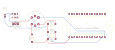
\includegraphics[width=0.5\textwidth]{assets/GasSense-brd}}}
	\caption{Το PCB κύκλωμα του GasSense.}
	\label{Το PCB κύκλωμα του GasSense.}
\end{figure}

Στο άνω PCB βλέπουμε την πλακέτα που σχεδιάστηκε μέσω του λογισμικού KiCad.

\subsection{LightSense}

\begin{figure}[H]
	\centerline{\includegraphics[width=0.5\textwidth]{assets/lightsense-schematic}}
	\caption{Το σχηματικό κύκλωμα του LightSense.}
	\label{Το σχηματικό κύκλωμα του LightSense.}
\end{figure}

Στο άνω σχηματικό βλέπουμε την συνδεσμολογία της συσκευής του LightSense. Η σύνδεση έχει γίνει με βάση έναν online οδηγό. \cite{ldrconnect}.

\begin{figure}[H]
	\colorbox{PineGreen}{\centerline{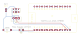
\includegraphics[width=0.5\textwidth]{assets/LightSense-brd}}}
	\caption{Το PCB του LightSense.}
	\label{Το PCB του LightSense.}
\end{figure}

Στο άνω PCB βλέπουμε την πλακέτα που σχεδιάστηκε μέσω του λογισμικού KiCad.

\subsection{TempSense}

\begin{figure}[H]
	\centerline{\includegraphics[width=0.5\textwidth]{assets/tempsense-schematic}}
	\caption{Το σχηματικό κύκλωμα του TempSense.}
	\label{Το σχηματικό κύκλωμα του TempSense.}
\end{figure}

Στο άνω σχηματικό βλέπουμε την συνδεσμολογία της συσκευής του TempSense. Η σύνδεση έχει γίνει με βάση έναν online οδηγό, συγκεκριμένα σε κατάσταση "Normal". \cite{mq6connect} Αξίζει να σημειωθεί ότι η αντίσταση στον αισθητήρα DS18B20 συνδέεται με το +5V λόγω της ανάγκης του πρωτοκόλλου 1-Wire για pull-up αντίσταση. Η συγκεκριμένη αντίσταση είναι απαραίτητη για να διασφαλιστεί ότι η γραμμή δεδομένων μπορεί να φτάσει στην υψηλή τάση, όταν δεν υπάρχει σήμα από τον αισθητήρα ή τον μικροελεγκτή. \cite{ds18b20connect}

\begin{figure}[H]
	\colorbox{PineGreen}{\centerline{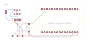
\includegraphics[width=0.5\textwidth]{assets/TempSense-brd}}}
	\caption{Το PCB του TempSense.}
	\label{Το PCB του TempSense.}
\end{figure}

Στο άνω PCB βλέπουμε την πλακέτα που σχεδιάστηκε μέσω του λογισμικού KiCad.

\section{Κώδικας}
Λόγω της πολυπλοκότητας του έργου, έχει χωριστεί σε μικρότερα έργα.

\begin{itemize}
	\item HomeSense-Platform: Το κεντρικό αποθετήριο το οποίο έχει ως sub-modules όλα τα σχετικά έργα του HomeSense το οποίο βρίσκεται στο \url{https://github.com/KostelidisDev/HomeSense-Platform}
	\item HomeSense-Presentation: Το αποθετήριο το οποίο περιέχει τον LaTeX κώδικα της παρουσίασης το οποίο βρίσκεται στο \url{https://github.com/KostelidisDev/HomeSense-Presentation}
	\item HomeSense-Document: Το αποθετήριο το οποίο περιέχει τον LaTeX κώδικα της εργασίας το οποίο βρίσκεται στο \url{https://github.com/KostelidisDev/HomeSense-Document}
	\item HomeSense: Το αποθετήριο το οποίο περιέχει τον κώδικα του API και του UI το οποίο βρίσκετε στο \url{https://github.com/KostelidisDev/HomeSense}
	\item HomeSense Deployer: Το αποθετήριο το οποίο περιέχει τον deployer για το API και το UI μέσω Docker Compose το οποίο βρίσκεται στο \url{https://github.com/KostelidisDev/HomeSense-Deployer}
	\item NodeSense: Το αποθετήριο το οποίο περιέχει τον template κώδικα των συσκευών το οποίο βρίσκεται στο \url{https://github.com/KostelidisDev/NodeSense}
	\item KiCadGrobotronics: Το αποθετήριο το οποίο περιέχει, custom library για τα components που αγοράστηκαν, από το κατάστημα GRobotronics, το οποίο βρίσκεται στο \url{https://github.com/IordanisKostelidis/KiCadGrobotronics}
	\item TempSense: Το αποθετήριο το οποίο περιέχει τον κώδικα, το σχηματικό και το PCB της συσκευής με τον αισθητήρα θερμοκρασίας το οποίο βρίσκεται στο \url{https://github.com/KostelidisDev/TempSense}
	\item LightSense: Το αποθετήριο το οποίο περιέχει τον κώδικα, το σχηματικό και το PCB της συσκευής με τον αισθητήρα φωτός το οποίο βρίσκεται στο \url{https://github.com/KostelidisDev/LightSense}
	\item GasSense: Το αποθετήριο το οποίο περιέχει τον κώδικα, το σχηματικό και το PCB της συσκευής με τον αισθητήρα αερίου το οποίο βρίσκεται στο \url{https://github.com/KostelidisDev/GasSense}
\end{itemize}

\section{Διάγραμμα Αλληλεπίδρασης Χρήστη-Συστήματος}
\begin{figure}[H]
	\centerline{\includegraphics[width=0.3\textwidth]{assets/diagram}}
	\caption{Διάγραμμα Αλληλεπίδρασης Χρήστη-Συστήματος}
	\label{Διάγραμμα Αλληλεπίδρασης Χρήστη-Συστήματος}
\end{figure}

\section{Συμπεράσματα}

Κατά τη διάρκεια της υλοποίησης του έργου, καταφέραμε να επιτύχουμε τον κύριο στόχο του συστήματος, ο οποίος ήταν η ασύρματη συλλογή και παρουσίαση δεδομένων από τρεις αισθητήρες μέσω ενός δικτύου WiFi και ενός Raspberry Pi. Η διαδικασία αυτή μας προσέφερε τη δυνατότητα να κατανοήσουμε καλύτερα τις εφαρμογές μικροελεγκτών, τις ασύρματες επικοινωνίες και την επεξεργασία δεδομένων.

Ωστόσο, η υλοποίηση δεν ήταν χωρίς προκλήσεις. Ένα από τα πιο δύσκολα σημεία ήταν η πλακέτα του αισθητήρα θερμοκρασίας (TempSense), καθώς αντιμετώπισα προβλήματα κατά το σχεδιασμό της αρχικής πλακέτας. Στην πρώτη έκδοση, τα τρία pins (+5V, value, GND) ήταν πολύ κοντά το ένα στο άλλο, με αποτέλεσμα να υπάρχει πρόβλημα σύνδεσης/soldering. Στη δεύτερη έκδοση, εντόπισα σχεδιαστικό λάθος, όπου αντί να συνδέσω την αντίσταση στο +5V, την είχα συνδέσει στο GND.

Ένα άλλο πρόβλημα προέκυψε με τον αισθητήρα αερίου (GasSense). Αρχικά, δεν ήξερα ακριβώς ποια αέρια ανιχνεύει, αλλά μετά από δοκιμές, διαπίστωσα ότι εντοπίζει αέρια παρόμοια με αυτά που χρησιμοποιούνται σε αναπτήρες.

Επιπλέον, αντιμετώπισα δυσκολίες με το soldering, καθώς ήταν η πρώτη φορά που ασχολήθηκα με τη διαδικασία. Στην αρχή, υπήρξαν αρκετά λάθη, όπως υπερβολική ποσότητα καλαι, λάθος θερμοκρασία στην μύτη κόλλησης, αλλά με την εμπειρία και τον χρόνο, το αποτέλεσμα βελτιώθηκε.

Από τα παραπάνω, το πιο σημαντικό συμπέρασμα είναι ότι το έργο μας απέδειξε πως με τη χρήση μικροελεγκτών και ασύρματης επικοινωνίας μπορούν να δημιουργηθούν πολλές χρήσιμες και καινοτόμες εφαρμογές. Επιπλέον, η υλοποίηση του συστήματος με βοήθησε να αποκτήσω γνώσεις και εμπειρίες σε τομείς στους οποίους δεν είχα εμβαθύνει στο παρελθόν (π.χ. διαιρέτες τάσεων), καθώς και να εξοικειωθώ με τη διαδικασία σχεδιασμού πλακετών μέσω του KiCad αλλά και το soldering.

\section{Σχετικά με το έργο}
Αυτό το έργο πραγματοποιήθηκε στο πλαίσιο του μαθήματος Ρ101: Ενσωματωμένα Συστήματα, στο μεταπτυχιακό πρόγραμμα στη Ρομποτική, που προσφέρεται από το Τμήμα Μηχανικών Πληροφορικής και Τηλεπικοινωνιών του Διεθνούς Πανεπιστημίου της Ελλάδος.

\begin{thebibliography}{00}
	\bibitem{resistorkit} “Carbon Film Αντιστάσεις Kit 0.25W (1τμχ) | Skroutz.gr,” www.skroutz.gr, 2025. https://www.skroutz.gr/s/28677532/Carbon-Film-Antistaseis-Kit-0-25W-1tmch.html (accessed Jan. 31, 2025).
	\bibitem{esp8266} “NodeMCU - Lua based ESP8266,” grobotronics.com, 2025. https://grobotronics.com/nodemcu-lua-based-esp8266.html (accessed Jan. 31, 2025).
	\bibitem{adc} “NodeMCU ADC with Arduino IDE” www.electronicwings.com, 2025. https://www.electronicwings.com/nodemcu/nodemcu-adc-with-arduino-ide (accessed Jan. 31, 2025).
	\bibitem{ds18b20-1wire} “ESP8266 DS18B20 Temperature Sensor with Arduino IDE (Single, Multiple, Web Server),” randomnerdtutorials.com, 2025. https://randomnerdtutorials.com/esp8266-ds18b20-temperature-sensor-web-server-with-arduino-ide/ (accessed Jan. 31, 2025).
	\bibitem{mq6} “LPG Gas Sensor - MQ-6,” grobotronics.com, 2025. https://grobotronics.com/lpg-gas-sensor-mq-6.html (accessed Jan. 31, 2025).
	\bibitem{ldr} “Photo resistor LDR 5mm,” grobotronics.com, 2025. https://grobotronics.com/photo-resistor-ldr-5mm.html (accessed Jan. 31, 2025).
	\bibitem{ds18b20} "Waterproof Temperature Sensor - DS18B20," grobotronics.com, 2025. https://grobotronics.com/waterproof-temperature-sensor-ds18b20.html (accessed Jan. 31, 2025).
	\bibitem{mss2235} "Slide Switch DPDT ON-ON 0.3A/6VDC," grobotronics.com, 2025. https://grobotronics.com/dpdt-on-on-0.3a-6vdc.html (accessed Jan. 31, 2025).
	\bibitem{dc2dc} "DC-DC Converter Step-Down 5V 1A," grobotronics.com, 2025. https://grobotronics.com/dc-dc-converter-step-down-5v-1a.html (accessed Jan. 31, 2025).
	\bibitem{bcv9} "Battery Clip 9V - Wires," grobotronics.com, 2025. https://grobotronics.com/battery-clip-9v-wires.html (accessed Jan. 31, 2025).
	\bibitem{bv9} "Battery 9V Varta Longlife Power - 550mAh," grobotronics.com, 2025. https://grobotronics.com/battery-9v-varta-longlife-550mah.html (accessed Jan. 31, 2025).
	\bibitem{rpi3b} "Raspberry Pi 3 Model B+ | Skroutz.gr," www.skroutz.gr, 2025. https://www.skroutz.gr/s/14311305/Raspberry-Pi-3-Model-B.html (accessed Jan. 31, 2025).
	\bibitem{miltimeter} "Uni-T UT131Β Ψηφιακό Πολύμετρο με Buzzer με Μέτρηση AC / DC / Αντίστασης | Skroutz.gr," www.skroutz.gr, 2025. https://www.skroutz.gr/s/14355908/Uni-T-UT131V-PSifiako-Polymetro-me-Buzzer-me-Metrisi-AC-DC-Antistasis.html (accessed Jan. 31, 2025).
	\bibitem{solderstation} "Andowl Q-GJ5 Βάση με Μεγενθυτικό Φακό Κολλητηριού | Skroutz.gr," www.skroutz.gr, 2025. https://www.skroutz.gr/s/30840110/Andowl-Q-GJ5-Vasi-me-Megenthytiko-Fako-Kollitiriou.html (accessed Jan. 31, 2025).
	\bibitem{solderingkit} "501610 Κολλητήρι Ρεύματος 60W με Ρύθμιση Θερμοκρασίας με Θήκη | Skroutz.gr" www.skroutz.gr, 2025. https://www.skroutz.gr/s/20534158/501610-Kollitiri-Reymatos-60W-me-Rythmisi-THermokrasias-me-THiki.html (accessed Jan. 31, 2025).
	\bibitem{mq6connect} "AirQualityMQ135 \ Learning \ Wiring," wiring.org.co, 2025. https://wiring.org.co/learning/basics/airqualitymq135.html (accessed Jan. 31, 2025).
	\bibitem{ldrconnect} "NodeMCU With LDR : 4 Steps (with Pictures) - Instructables" www.instructables.com, 2025. https://www.instructables.com/NodeMCU-With-LDR/ (accessed Jan. 31, 2025).
	\bibitem{ds18b20connect} "DS18B20: Programmable Resolution 1-Wire Digital Thermometer Data Sheet (Rev.6)" www.analog.com, 2025. https://www.analog.com/media/en/technical-documentation/data-sheets/DS18B20.pdf (accessed Jan. 31, 2025).
\end{thebibliography}


\end{document}